\section{CONCLUSIONES}

En resumen al estado de la cuestión se puede observar que a lo largo de la historia se han desarrollado múltiples tecnologías para facilitar y mejorar las condiciones de vida en el hogar a través de tecnología.

A día de hoy existen proyectos para dotar de inteligencia a los frigoríficos, sin embargo, solamente son prototipos debido a su alto coste de fabricación.

\begin{figure}[h!]
    \centering
    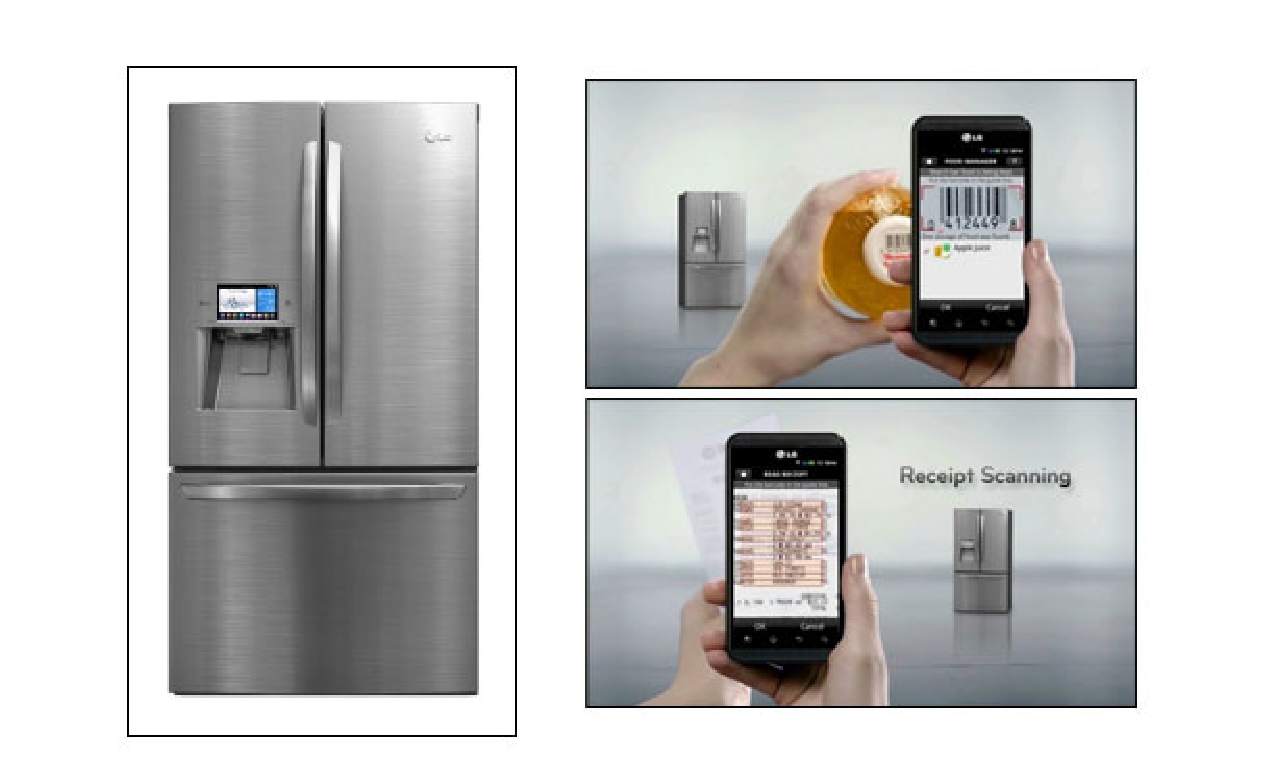
\includegraphics[keepaspectratio,width=0.6\textwidth]{frigo-lg.eps}
    \label{fig:frigo-lg}
\end{figure}

Para traer al hogar parte de esta tecnología se ha aprovechado de los avances en hardware libre (a través de Arduino) para desarrollar un prototipo de frigorífico inteligente. Este protipo tendrá como objetivo dotar de inteligencia al frigorífico sin tener que realizar una gran inversión en hardware.